\documentclass{beamer}

\usepackage{graphicx}
\usepackage{hyperref}
\usepackage[latin1]{inputenc}
\usepackage[T1]{fontenc}
\usepackage[english]{babel}
\usepackage{listings}
\usepackage{xcolor,mathrsfs,url}
\usepackage{amssymb}
\usepackage{amsmath}
\usepackage{ifthen}

\usepackage{metricsbeamer} % using the metric beamer style

% The command to define a subsection is '\subsec{}' and NOT '\subsection'.
% This code generates the bar. Don't edit.
\newcommand{\midbarnew}{}
\newcommand{\subsec}[1]
{
  \ifthenelse{\equal{#1}{}}
  {\renewcommand{\midbarnew}{} \subsection{}}
  {\renewcommand{\midbarnew}{ $\mid$ } \subsection{#1}}
}

% change the pictures here, if necessary. logobig and logosmall are the internal names
% for the pictures: do not modify them, just change "hulogo" and "logo". Pictures must be 
% supplied as JPEG, PNG or PDF
%########################################

\pgfdeclareimage[height=2cm]{logobig}{logo} % use hucase instead for the Humboldt-Case Logo
\pgfdeclareimage[height=1cm]{logosmall}{logo}

% use this number to modify the scaling of the headline on titlepage
\def\titlescale{1.0}


\def\authora{Battista Severgnini}	% First Author
\def\affa{Department of Economics-CBS} % First Author's Affiliation
\def\authorb{}  % Second Author
\def\affb{} % Second Author's Affiliation
\def\authorc{}  % Third Author
\def\affc{} % Third Author's Affiliation
\def\linka{}	% Link to your institution's/ personal website
\def\linkb{}
\def\linkc{}\def\email{\href{mailto:bs.eco@cbs.dk}{bs.eco@cbs.dk}}	% Your email address

\title[Price Levels and the Exchange Rate in the Long Run.]{International Economics - B.Sc. IB\\ 10. Open-Economy Macroeconomics: \\Price Levels and the Exchange Rate in the Long Run
 \\  \footnotesize{May $12^{th}$, 2014}}
\institute{Economics Department CBS}
%Start of the document
\begin{document}


\frame[plain]{% create the titleslide, layout controlled in metricsbeamer
	\titlepage
}

\Section{Plan for Today}

\frame{% how to print
\frametitle{Plan for Today}
Chapter 16:
\begin{itemize}
\item The law of one price
\item Purchasing power parity
\item A long-run exchange rate
model based on PPP
\item The Fisher effect
\item A General Model of Long-Run
Exchange Rates
\end{itemize}
}


\Section{Chapter 16. The Law of One Price}
\frame{% how to print
\frametitle{}
\begin{center}
\textcolor{blue}{\Huge{\textbf{Chapter 16: Price Levels and the Exchange Rate in the Long Run
}}}
\end{center}
}


\frame{
\frametitle{The Law of One Price (1)}
The prices of identical goods sold in different
countries must be the same when expressed
in terms of the same currency.
\begin{itemize}
\item  This law applies only in competitive markets
free of transport costs and official barriers to
trade.
\item Example: If the dollar/pound exchange rate
is USD 1.50 per pound, a sweater that sells for
USD 45 in New York must sell for Pound 30 in London.
\end{itemize}
}


\frame{
\frametitle{The Law of One Price (2)}
The dollar price of good i is the same wherever it
is sold
\begin{center}
$P^{i}_{US} = \left(E_{USD/EURO}\right) x \left(P^{i}_{E}\right)$
\end{center}
where:
\begin{itemize}
\item $P^{i}_{US}$ is the dollar price of good i when sold in
the U.S.
\item $P^{i}_{E}$ is the corresponding euro price in Europe
\item $\left(E_{USD/EURO}\right)$ is the dollar/euro exchange rate
\end{itemize}}

\Section{Chapter 16. Purchasing Power Parity}

\frame{
\frametitle{Purchasing Power Parity  (PPP)(1)}
PPP 
\begin{itemize}
\item is the application of the law of one price across countries for \textit{all} goods and services.
\item compares average prices across countries
\item predicts a dollar/euro exchange rate of
\begin{center}
$ E_{USD/EURO} =\frac{P_{US}}{P_{E}}$
\end{center}
where
\begin{itemize}
\item $P_{US}$ is the dollar price of a reference commodity
basket sold in the United States
\item $P_{E}$ is the euro price of the same basket in Europe
\end{itemize}
\end{itemize}
}

\frame{
\frametitle{Purchasing Power Parity (PPP)(2)}
Rearranging,
\begin{center}
$ P_{US}=\left(E_{USD/EURO}\right)x\left(P_{E}\right)$
\end{center}
All countries' price levels are equal when measured in
terms of the same currency
}

\frame{
\frametitle{PPP \& Law of One Price}
\begin{itemize}
\item The law of one price applies to individual
commodities; PPP applies to the general
price level
\item If the law of one price holds true for every
commodity $\Rightarrow$ PPP must hold for the same
reference baskets across countries
\item BUT if PPP holds, this does not mean that law of one price is respected
\end{itemize}
}


\frame{
\frametitle{Purchasing Power Parity (PPP)(3)}
\begin{enumerate}
\item Absolute PPP: exchange rates equal relative price levels
\item Relative PPP: the percentage change in the exchange
rate between two currencies equals the difference
between the percentage changes in national price
levels.
\begin{center}
$\frac{\left(E_{USD/EURO,t} - E_{USD/EURO,t-1}\right)}{ E_{USD/EURO,t-1}}= \pi_{US, t} - \pi_{E, t}$
\end{center}
\end{enumerate}
where $\pi_{t}$ = inflation rate from period $t-1$ to $t$
}


\frame{
\frametitle{Absolute \& Relative PPP (1)}
If absolute PPP holds $\Rightarrow$ relative PPP holds
\begin{table}
\begin{center}
\begin{tabular}{||c|c|c||}\hline
 & $t-1$ & $t$ \\\hline
Absolute & $P_{US,t-1}=USD 100$ & $P_{US,t}= USD110$ \\ 
PPP      & $E_{t-1}P_{E,t-1}=USD100$ & $E_{t}P_{E,t} = USD110$ \\ \hline
\multicolumn{3}{||c||}{$\Rightarrow$} \\ \hline
Relative & \multicolumn{2}{|c||}{$\pi_{US, t-1}=10\%$}\\
PPP      & \multicolumn{2}{|c||}{$\pi_{E, t-1}=\frac{\left(E_{t} - E_{t-1}\right)}{ E_{t-1}}$}\\\hline \hline
\end{tabular}
\end{center}
\end{table}
}


\frame{
\frametitle{Absolute \& Relative PPP (2)}
\textbf{Not the other way around!}
\begin{table}
\begin{center}
\begin{tabular}{||c|c|c||}\hline
 & $t-1$ & $t$ \\\hline
Relative & \multicolumn{2}{|c||}{$\pi_{US, t}=10\%$}\\
PPP      & \multicolumn{2}{|c||}{$\pi_{E, t}=\frac{\left(E_{t} - E_{t-1}\right)}{ E_{t-1}}$} \\\hline
\multicolumn{3}{||c||}{NOT TRUE $\Rightarrow$} \\ \hline
Absolute & $P_{US,t-1}=USD 200$ & $P_{US,t-1}= USD220$ \\ 
PPP      & $E_{t-1}P_{E,t-1}=USD100$ & $E_{t}P_{E,t} = USD110$ \\ \hline \hline
\end{tabular}
\end{center}
\end{table}
}


\Section{Chapter 16. A Long-Run Exchange Rate
Model Based on PPP}


\frame{
\frametitle{A Long-Run Exchange Rate
Model Based on PPP}
\begin{itemize}
\item Monetary approach to the exchange rate
\item A theory of how exchange rates and
monetary factors interact in the long run.
\item The fundamental equation of the monetary
approach
\item Price levels can be expressed in terms of
domestic money demand and supplies.
\end{itemize}
\begin{enumerate}
\item In the United States:
\begin{center}
$P_{US}= \frac{M^{s}_{US}}{L \left(R_{USD}, Y_{US}\right)}$
\end{center}
\item In Europe:
\begin{center}
$P_{E}= \frac{M^{s}_{E}}{L \left(R_{EURO}, Y_{E}\right)}$
\end{center}
\end{enumerate}}


\frame{
\frametitle{PPP and Money Market}
\begin{center}
$E_{USD/EURO}=\frac{P_{US}}{P_{E}}=\frac{\frac{M^{s}_{US}}{L \left(R_{USD}, Y_{US}\right)}}{\frac{M^{s}_{E}}{L \left(R_{EURO}, Y_{E}\right)}}$
\end{center}
Specific Predictions:
\begin{enumerate}
\item Money supplies: if $M^{s}_{US} \left(M^{s}_{EU}\right) \Uparrow \Rightarrow$ long-run depreciation (appreciation) of the dollar against the euro
\item interest rates: if $R_{USD} \left(R_{EU}\right) \Uparrow \Rightarrow$  
causes a depreciation (appreciation) of the dollar against the
euro
\item Output levels: a rise if $Y_{US} \left(Y_{E}\right) \Uparrow \Rightarrow$ causes an appreciation
(depreciation) of the dollar against the euro.
\end{enumerate}
}


\Section{Chapter 16. The Fisher Effect}

\frame{
\frametitle{The Fisher Effect (1)}
\begin{itemize}
\item A more reasonable description of
monetary policy is constantly growing
money supply
\item Money supply grows at a constant
growth rate results in ongoing inflation
at the same rate
\end{itemize}
}

\frame{
\frametitle{The Fisher Effect (2)}
\begin{center}
$E_{USD/EURO}=\frac{P_{US}}{P_{E}}=\frac{\frac{M^{s}_{US}}{L \left(R_{USD}, Y_{US}\right)}}{\frac{M^{s}_{E}}{L \left(R_{EURO}, Y_{E}\right)}}$
\end{center}
Given $M^{s}_{E}$ and $P_{EURO}$ constant, if $M^{s}_{US}$ grows by $\pi$, $P_{US}$ grows by $\pi_{US}$
\begin{center}
$\Rightarrow$
\end{center}
\begin{center}
$E$ depreciated by $\pi$ each period
\end{center}
\begin{center}
$\frac{E_{USD/EURO,t}-E_{USD/EURO,t-1}}{E_{USD/EURO, t}}=\pi_{US,t}-\pi_{US,t-1}$
\end{center}
Monetary policies in
the US and Euroland determine the
development in the exchange rate
}


\frame[plain]{
\frametitle{The Fisher Effect (3)}
Given Uncovered Interest Rate Parity,
\begin{center}
$R_{USD,t}= R_{EURO,t}+\left(\frac{E^{e}_{USD/EURO,t+1}-E_{USD,/EUROt}}{E_{USD/EURO,t}}\right)$
\end{center}
and relative PPP
\begin{center}
$\frac{\left(E_{USD/EURO,t} - E_{USD/EURO,t-1}\right)}{ E_{USD/EURO,t-1}}= \pi_{US, t} - \pi_{E, t}$
\end{center}
\begin{center}
$\Rightarrow$
\end{center}
Real interest rates are equal
\begin{center}
$\Rightarrow$
\end{center}
\begin{center}
$R_{USD} - R_{EURO} = \pi^{e}_{US} - \pi^{e}_{E}$
\end{center}
or
\begin{center}
$R_{USD} - \pi^{e}_{US} = R_{EURO}- \pi^{e}_{E}$
\end{center}
}



\frame{
\frametitle{The Fisher Effect (4)}
\begin{itemize}
\item A rise (fall) in a country's expected
inflation rate will eventually cause an
equal rise (fall) in the interest rate that
deposits of its currency offer.
\item In the long run, purely monetary
developments should have no real
effects.
\item expected growth in money
supply affects the interest rate
through inflation.
\end{itemize}
}

\frame{
\frametitle{Interest and Monetary Policy (1)}
\begin{itemize}
\item If growth in $M^{s}_{US}$ changes permanently
from $\pi$ to $\pi+\Delta\pi$ (and $M^{s}_{E}$ is constant)
such that $\pi_{US, t}$ and $\pi^{e}_{US}$ increases
from $\pi$ to $\pi+\Delta\pi$
\item $R_{US}$ increases by $\delta\pi$ (and $R_{e}$ is
unchanged)
\end{itemize}
}

\frame{
\frametitle{Interest and Monetary Policy (2)}
\begin{itemize}
\item If $R_{US} \Uparrow \Rightarrow L\left(R_{US}, Y_{US}\right) \Downarrow \Rightarrow E_{US/EURO} \Uparrow$
\end{itemize}
\begin{center}
$\Uparrow E_{US/EURO}=\frac{P_{US}}{P_{E}}=\frac{M^{S}_{US}L\left(R_{EURO}, Y_{E}\right)}{M^{S}_{E}L\left(R_{US}, Y_{US}\right)\Downarrow}$
\end{center}
}




\frame[plain]{
\frametitle{Fig. 16-1: Long-Run Time Paths of U.S. Economic Variables After a Permanent Increase in the Growth Rate of the U.S. Money Supply}
\begin{figure}
	\centering
		\includegraphics[width=0.85\textwidth]{151.pdf}
	\label{fig:11}
\end{figure}
}


\frame[plain]{
\frametitle{Fig. 16-1: Long-Run Time Paths of U.S. Economic Variables After a Permanent Increase in the Growth Rate of the U.S. Money Supply}
\begin{figure}
	\centering
		\includegraphics[width=0.85\textwidth]{151b.pdf}
	\label{fig:11}
\end{figure}
}

\frame[plain]{
\frametitle{Fig. 16-1: Long-Run Time Paths of U.S. Economic Variables After a Permanent Increase in the Growth Rate of the U.S. Money Supply}
\begin{figure}
	\centering
		\includegraphics[width=0.85\textwidth]{151c.pdf}
	\label{fig:11}
\end{figure}
}

\Section{Chapter 16. Empirical Evidence on PPP}

\frame{
\frametitle{Empirical Evidence on PPP (1)}
\begin{itemize}
\item The empirical support for PPP and
the law of one price is weak.
\item The prices of identical commodity
baskets, when converted to a single
currency, differ substantially across
countries.
\item Relative PPP also performs poorly.
\end{itemize}}


\frame[plain]{
\frametitle{Fig. 16-2: The Yen/Dollar Exchange Rate and Relative Japan-U.S. Price Levels, 1980-�2006}
\begin{figure}
	\centering
		\includegraphics[width=0.85\textwidth]{152.pdf}
	\label{fig:11}
\end{figure}
}


\frame[plain]{
\frametitle{Figure: Empirical Evidence of PPP (1)}
\begin{figure}
	\centering
		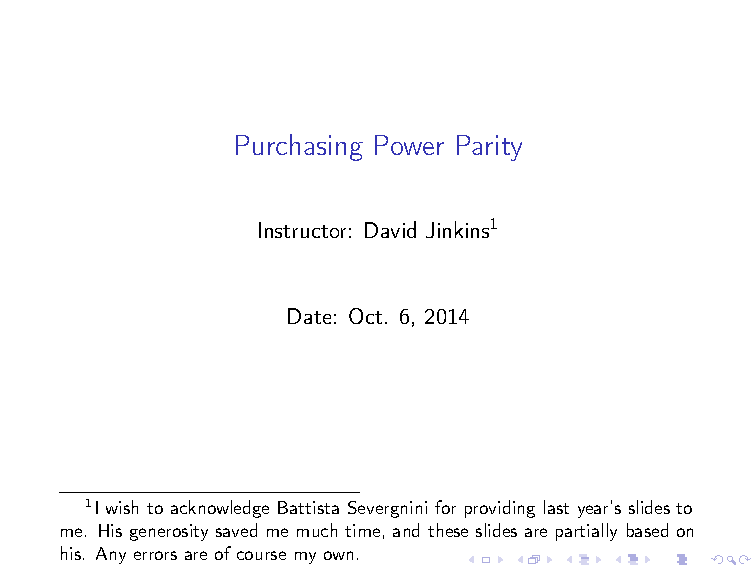
\includegraphics[width=0.85\textwidth]{ppp.pdf}
	\label{fig:11}
\end{figure}
}


\frame[plain]{
\frametitle{Figure: Empirical Evidence of PPP (2)}
\begin{figure}
	\centering
		\includegraphics[width=0.85\textwidth]{hyper.pdf}
	\label{fig:11}
\end{figure}
}

\frame[plain]{
\frametitle{Figure: The Big Mac Index}
\begin{figure}
	\centering
		\includegraphics[width=0.85\textwidth]{bigmac.pdf}
	\label{fig:11}
\end{figure}
}

\frame{
\frametitle{Reasons}
\begin{enumerate}
\item Trade barriers and non-tradable products 
\item Imperfect competition
\item Differences in measures of average prices for baskets of goods and services
\end{enumerate}
}

\Section{Chapter 16. A General Model of Long-Run
Exchange Rates}

\frame{
\frametitle{A General Model of Long-Run
Exchange Rates (1)}
The Real Exchange Rate
\begin{itemize}
\item Measure of the prices of one country's
goods and services relative to the other's.
\item The real exchange rate is the dollar price of
the European basket relative to that of the
US price:
\begin{center}
$q_{USD/EURO} = \frac{\left(E_{USD/EURO} x P_{E}\right)}{P_{US}}$
\end{center}
\item Observe that PPP only holds for $q_{USD/EURO}=1$
(absolute) or $q_{USD/EURO,t}-q_{USD/EURO,t-1}=0$ (conditional)
\end{itemize}}

\frame{
\frametitle{A General Model of Long-Run
Exchange Rates (2)}
\begin{enumerate}
\item Real depreciation (q increases): If US
prices fall in relation to foreign prices
(measured in USD). This happens if:
\begin{itemize}
\item Nominal exchange rate depreciates (E
increases), or
\item US prices fall, or
\item Euroland prices increase
\end{itemize}
\item Real appreciation (q falls): If US prices
increases relative to foreign prices
(measured in USD). This happens if:
\begin{itemize}
\item Nominal exchange rate appreciates (E falls),
or
\item US prices increase, or
\item Euroland prices fall
\end{itemize}
\end{enumerate}
}



\frame{
\frametitle{A General Model of Long-Run
Exchange Rates (3)}
We can express the nominal exchange
rate as:
\begin{center}
$E_{USD/EURO} = q_{USD/EURO} x (\frac{P_US}{P_E})$
\end{center}
\begin{center}
$\Rightarrow$
\end{center}
\begin{center}
$\frac{q^{e}_{USD/EURO}-q_{USD/EURO}}{q_{USD/EURO}}=\frac{E^{e}_{USD/EURO}-E_{USD/EURO}}{E_{USD/EURO}}-\left(\pi^{e}_{US}-\pi^{e}_{EURO}\right)$
\end{center}
Combining with the interest parity condition, the international interest gap is equal to:
\begin{center}
$\frac{q^{e}_{USD/EURO}-q_{USD/EURO}}{q_{USD/EURO}}=\frac{E^{e}_{USD/EURO}-E_{USD/EURO}}{E_{USD/EURO}}-\left(\pi^{e}_{US}-\pi^{e}_{EURO}\right)$
\end{center}
\begin{center}
$R_{US}-R_{EURO}=\frac{q^{e}_{USD/EURO}-q_{USD/EURO}}{q_{USD/EURO}}-\left(\pi^{e}_{US}-\pi^{e}_{EURO}\right)$
\end{center}
}


\frame[plain]{
\frametitle{Fig. 16-4: Determination of the Long-Run Real Exchange Rate}
\begin{figure}
	\centering
		\includegraphics[width=0.85\textwidth]{154.pdf}
	\label{fig:11}
\end{figure}
}


\frame[plain]{
\frametitle{}
\begin{figure}
	\centering
		\includegraphics[width=0.85\textwidth]{155.pdf}
	\label{fig:11}
\end{figure}
}

\frame{
\frametitle{Real Interest parity}
\begin{center}
$r^{e}_{US} -� r^{e}_{EU} = \frac{\left(q^{e}_{US/EU} -q_{US/EU}\right)}{q_{US/EU}}$
\end{center}
This equation is called real interest parity.
It says that differences in real interest rates (in terms of goods and services that are earned or forgone when lending or borrowing) between countries are equal to the expected change in the value/price/cost of goods and services between countries.
}

\end{document}
